\documentclass[../../thesis.tex]{subfiles}
\graphicspath{{./resources/} }
\begin{document}



\section{Configurable Software Systems}
Almost all software systems in use today are configurable. This means, almost all software systems
allow a user to customize the software system to their specific requirements.
To allow for such customizability, software systems provide a number of configuration options,
also called features, to specify the desired behaviour of the software system.
A feature is an attribute of a system that directly affects end-users \cite{kang1990feature}.
Each combination of configuration options describes a variant of the software system, making configurable software systems similar to
Software Product Lines (SPL) \cite{siegmund2012spl}.
For example, a web server like the Apache HTTP Server, allows the user to select features like 
compression, encryption or the use of
specific transport protocols like HTTP/2.

Features usually satisfy functional requirements \cite{siegmund2012spl} of users. Functional requirement as described
by \Citeauthor{malan2001functional} "[...] capture the intended behaviour of the system - or what the system will do".
Meaning, for the example of the webserver, a functional requirement would be the use of a specific compression algorithm like
Brotli\footnote{Brotli is a compression algorithm developed by Google primarily used by web servers to compress HTTP content. }.
On the other hand, software systems also have non-functional requirements. \Citeauthor{mylopoulos1992representing} describes non-functional
requirements as  "[...] requirements on its development or operational cost, performance, reliability,
maintainability, portability, robustness, and the like."

In this work, non-functional requirements, like performance or memory usage, of a software system are analyzed in regard to the configurations used.
Usually, the effect of configuration options on functional properties of the software are well documented and understood,
but the effect on non-functional properties are unknown to the user and more often than not, to the developer.


\subsubsection{Feature models} \label{sec:basics:feature_model}
Feature models, introduced by \Citet{kang1990feature}, serve as a mean to convey information about the features of a system.
Which features can be chosen and how those features can be combined. For this, the structural relationship between features is described.
Each feature can either be optional or mandatory and each feature can have child features that are either in an or group or an alternative group.
In an alternative group, only one of the child features can be selected, in an or group, at least one of the child features must be selected.
There are also composition rules, also known as cross-tree constraints, which define constraints not expressible in the hierarchical structure
of the features.

Feature models can be represented visually by feature diagrams or textually by formats like SXFM \cite{mendonca2009splot}.
Feature diagrams are an intuitive way for a user to work with feature models, they visualize the feature model in a tree diagram.
An example of a feature diagram can be seen in \autoref{fig:feature_diagram_example}. There, the features of an exemplary web server are described.
The web server has 4 features, of which 3 are optional and one is mandatory. It also includes two cross-tree constraints.
The feature \textit{Encryption} is an optional feature, without any constraints on it. This feature can be enabled or disabled however the
user likes. In this work, this kind of feature without any constraints on it is also referenced as an independent feature.
Even though the \textit{Keep\_alive} feature has no differences in the hierarchical structure to the \textit{Encryption} feature, it
has a cross-tree constrain. This constraint mandates, that if \textit{Keep\_alive} is selected, the \textit{HTTP/1} feature is selected too, since the
\textit{Keep\_alive} functionality is only available in the HTTP/1 protocol.
\textit{Compression} and \textit{Protocol} are both features with child features. Since \textit{HTTP/1} and \textit{HTTP/2} are in an
alternate group, only one of these two protocols can be chosen for a valid configuration.
With \textit{Compression}, one or both of the child features can be chosen, since they are in an or group.

\begin{figure}[]
  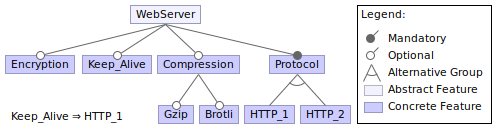
\includegraphics[width=1\textwidth]{feature_diagrams/example_feature_diagram.png}
  \caption[Feature diagram - exemplary web server]{
    Feature diagram of an exemplary web server created with FeatureIDE
  }\label{fig:feature_diagram_example}
\end{figure}




% \subsubsection{Constrains}
\subsubsection{Interactions}

Features in a software system directly influence the way a system behaves with respect to its functional and non-functional properties.
If we turned on the feature \textit{Encryption} in our exemplary web server, the webserver would need to encrypt the sent data.
This not only has impacts on the functional properties of the web server, but it also impacts the non-functional property.
The web server now has to further process the data before sending it, which results in more computational power needed.
The same goes for the feature \textit{Compression}, or more  specifically for the features \textit{Brotli} and \textit{Gzip}.
If the compression is enabled in the webserver, the webserver needs to compress the data before sending it, which
requires more computational power.

One could now assume, that if we enable both features at the same time, the computational power needed to process a request
is the sum of the power needed if the encryption is enabled and if the compression is enabled.
A more likely scenario would be, that the computational power needed would be less than that.
If we first compress the data, the encryption part of the webserver has to encrypt fewer data.
The two features \textit{Encryption} and \textit{Compression} interact.




\end{document}